\documentclass[10pt]{beamer}

\usetheme{default}

\usepackage[utf8]{inputenc}
\usepackage[russian]{babel}
\usepackage[OT1]{fontenc}
\usepackage{amsmath}
\usepackage{amsfonts}
\usepackage{amssymb}
\usepackage{graphicx}
\usepackage{etoolbox}
\usepackage{caption}
\usepackage{subcaption}
\usepackage{pifont}
\usepackage{xcolor}
\usepackage{framed}
\definecolor{shadecolor}{cmyk}{0,0,0,1}
\usepackage{listings}

\lstset{
	backgroundcolor=\color{lightgray},
	commentstyle=\color{blue},
	frame=single
	breakatwhitespace, 
	language=python, 
	columns=fullflexible, 
	keepspaces, 
	breaklines, 
	tabsize=3, 
	showstringspaces=false, 
	extendedchars=true,
	numbers=left
}

\makeatletter

\setbeamercolor{title}{fg=white}
\setbeamercolor{frametitle}{fg=black}
\setbeamerfont*{title}{family=\sffamily,size=\LARGE}

\setbeamerfont{page number in head/foot}{size=\scriptsize}
\setbeamertemplate{footline}[frame number]
\let\otp\titlepage
\renewcommand{\titlepage}{\otp\addtocounter{framenumber}{-1}}

\setbeamertemplate{background canvas}{%
	\ifnumequal{\c@framenumber}{0}{%
      
\includegraphics[width=\paperwidth,height=\paperheight]{images/cover.png}
   }{%
      \ifnumequal{\c@framenumber}{\inserttotalframenumber}{
         
\includegraphics[width=\paperwidth,height=\paperheight]{images/back.png}
      }{%
         % Other frames
      }%
   }%
}

\makeatother

\beamertemplatenavigationsymbolsempty

\author{Николай Анохин}
\title{\newline \newline \newline Лекция 2 \\ Задачи кластеризации}

\begin{document}

\defverbatim[colored]\kmeans{%
\begin{lstlisting}[tabsize=4,basicstyle=\ttfamily]
function kmeans(X, K):
	initialize N # number of objects
	initialize Mu = (mu_1 ... mu_K) # random centroids
	do:
		# E step
		for k in 1..K:
			for x in 1..N:
				compute r_nk # Cluster assignment
		# M step
		for k in 1..K:
			recompute mu_k # Update centroids
	until Mu converged
	J = loss(X, Mu)
	return Mu, J
\end{lstlisting}
}

\begin{frame}[plain]
\titlepage
\end{frame}

\begin{frame}{План занятия}
\tableofcontents
\end{frame}

% =======================
\section{Задача кластеризации}
% =======================

\begin{frame}{Задача кластеризации}

В задачах кластеризации целевая переменная не задана. Цель -- отыскать ``скрытую структуру'' данных.

\vspace{1em}
Зачем вообще рассматривать задачи без целевой переменной?
\begin{enumerate}
\item разметка данных -- дорогое удовольствие
\item можно сначала поделить, а потом разметить
\item возможность отслеживать эволюционные изменения
\item построение признаков
\item exploratory data analysis
\end{enumerate}

\end{frame}

\begin{frame}{Программисты python в Twitter}

\begin{center}
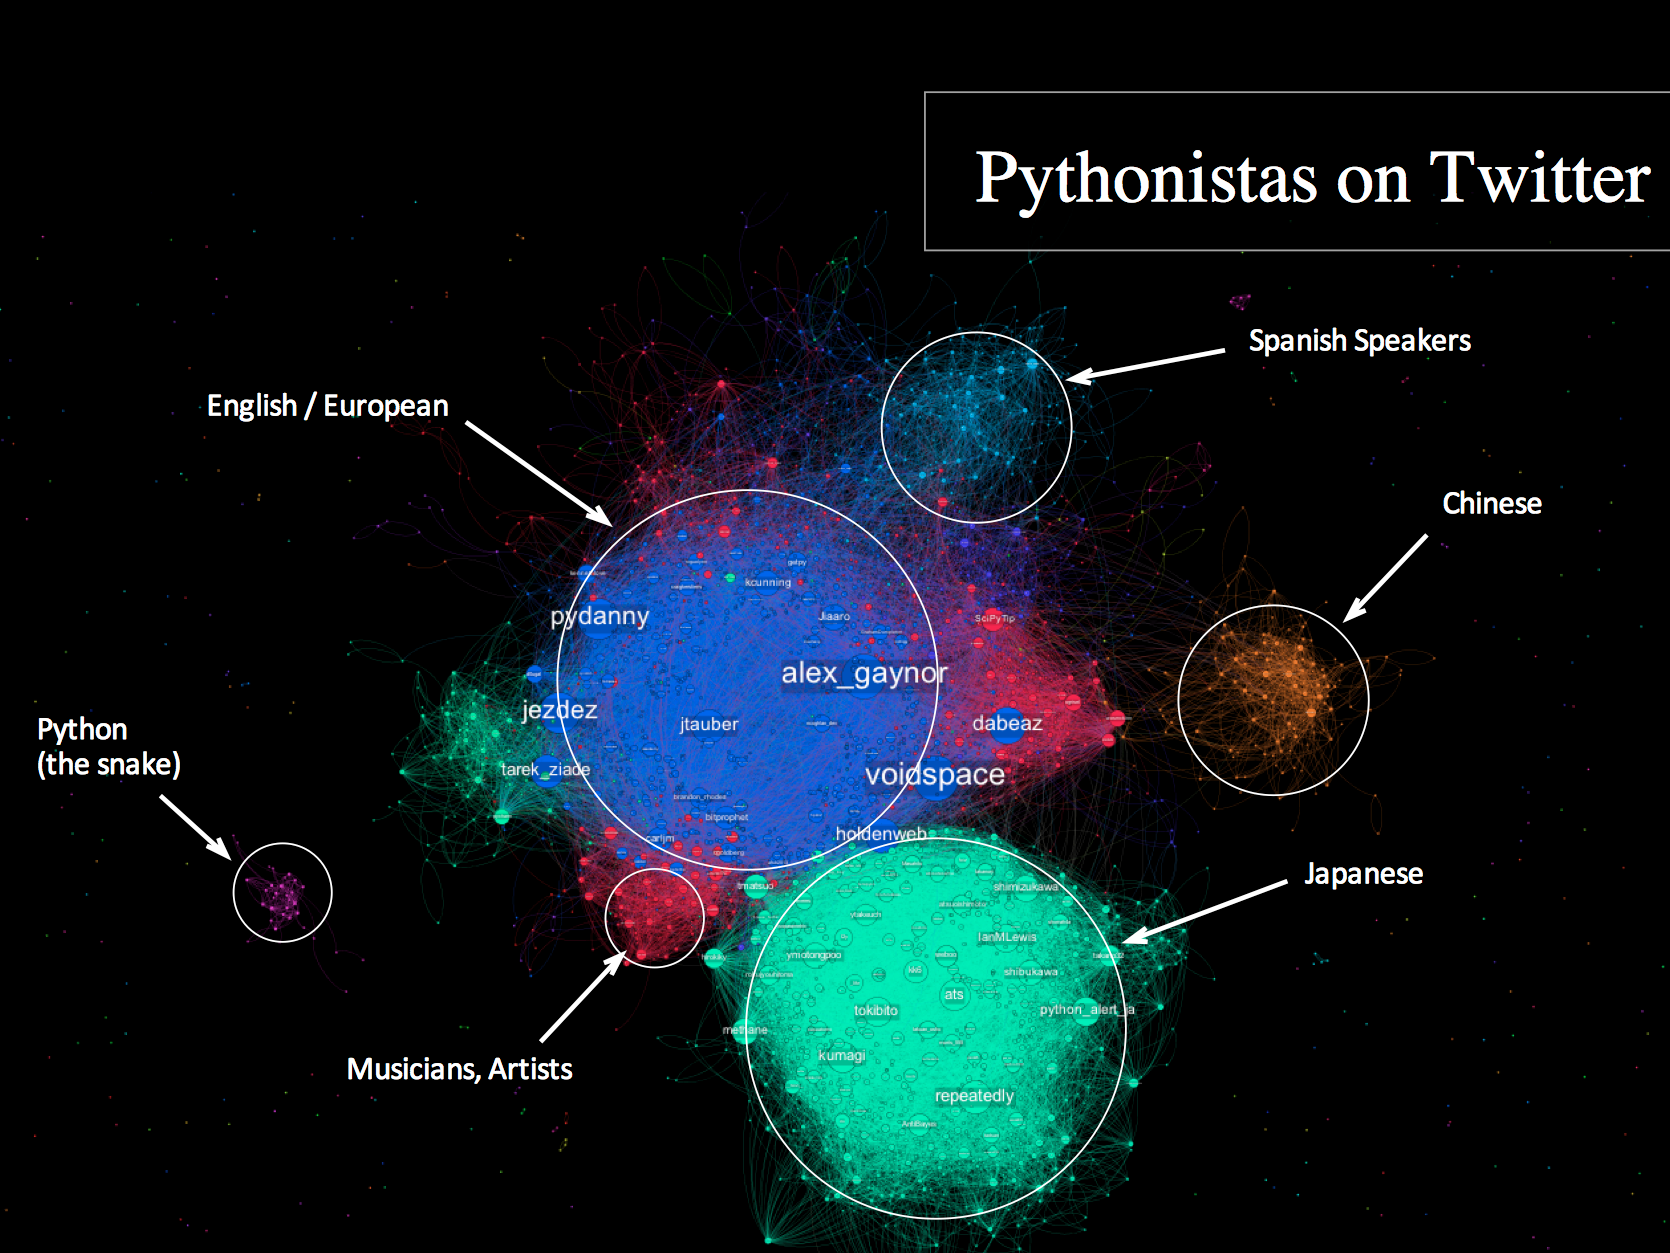
\includegraphics[scale=0.15]{images/python.png}
\end{center}
Графо-теоретические методы
(\href{http://giladlotan.com/2012/11/mapping-twitters-python-data-science-communities/}{источник})

\end{frame}

\begin{frame}{Похожие тематики}

\begin{center}
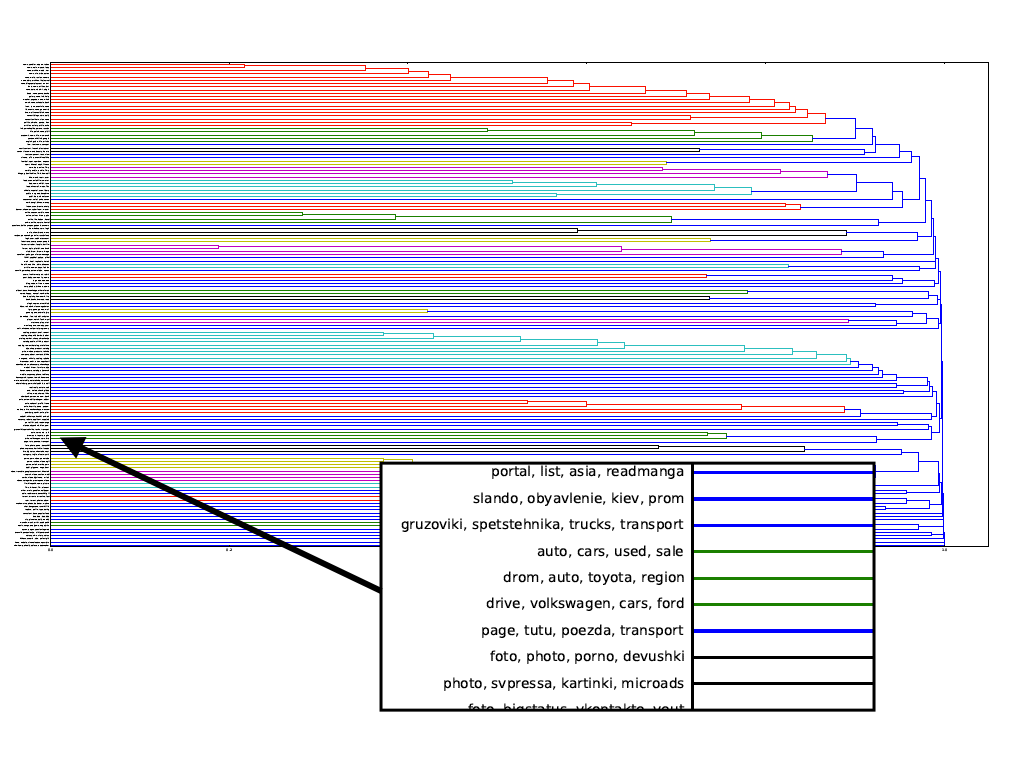
\includegraphics[scale=0.25]{images/hier.png}
\end{center}
Иерархическая кластеризия

\end{frame}

\begin{frame}{Топ 1000 самых посещаемых доменов рунета}

\begin{center}
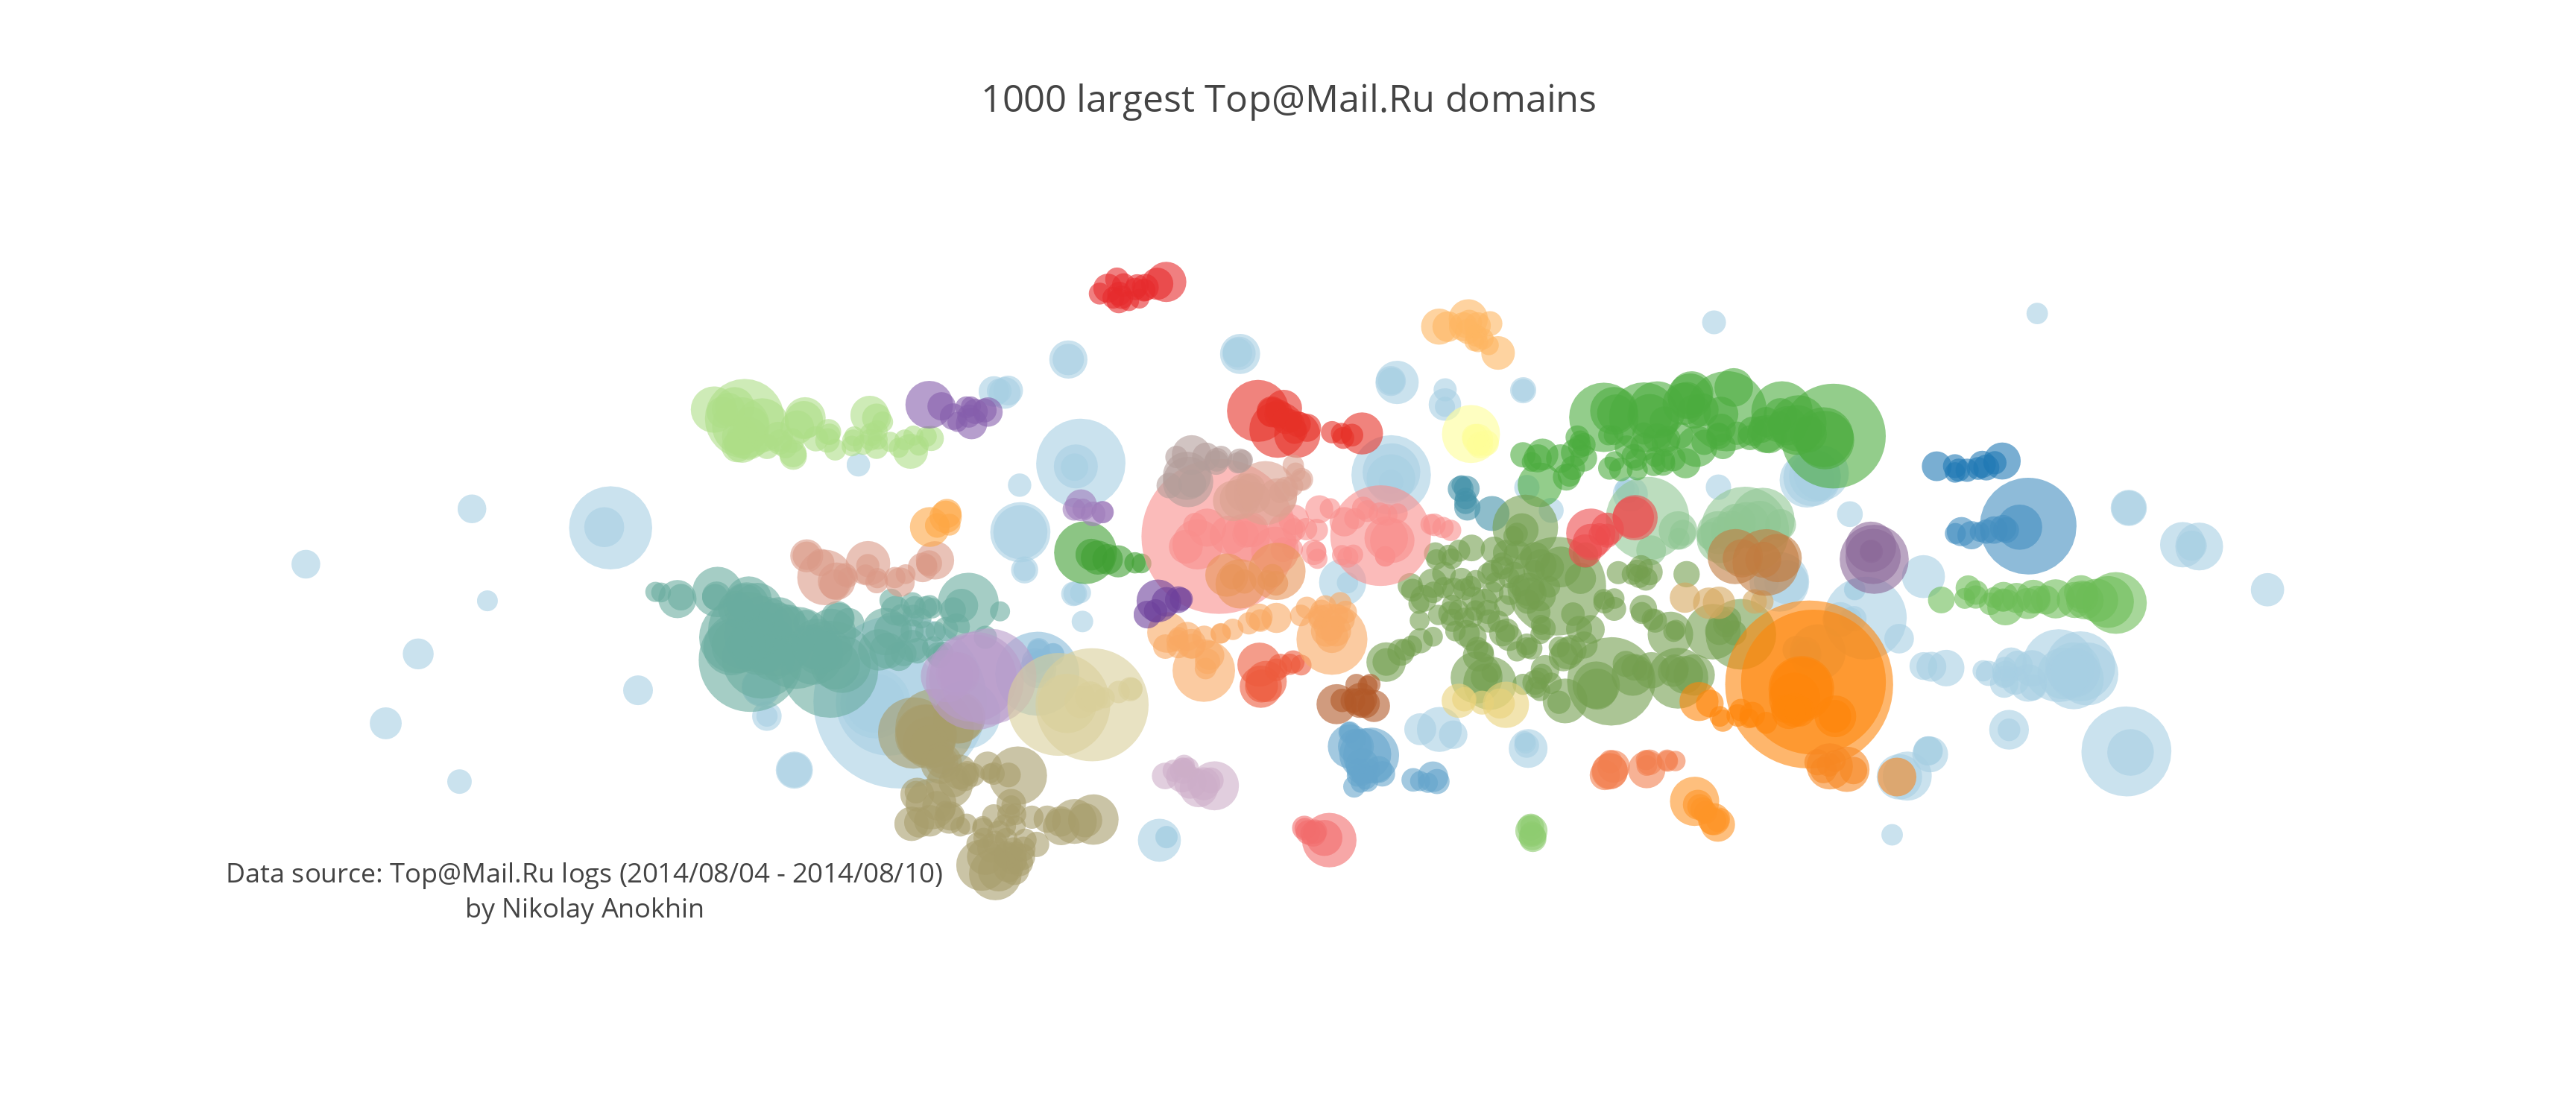
\includegraphics[width=\textwidth]{images/domains.png}
\end{center}
T-SNE + DBSCAN

\end{frame}

\begin{frame}{Постановка задачи}

{\bf Дано.} $N$ обучающих $D$-мерных объектов $\mathbf{x}_i \in \mathcal{X}$, образующих тренировочный набор данных (training data set) $X$.

\vspace{1em}
{\bf Найти.} Модель $h^*(\mathbf{x})$ из семейства параметрических функций $H = \{h(\mathbf{x, \mathbf{\theta}}): \mathcal{X} \times \Theta \rightarrow \mathbb{N}\}$, ставящую в соответствие произвольному $\mathbf{x} \in \mathcal{X}$ один из $K$ кластеров так, чтобы объекты внутри одного кластера были похожи, а объекты из разных кластеров различались.

\vspace{1em}
\begin{itemize}
\item Как определить похожесть объектов?
\item Как оценить качество модели?
\item Как выбрать $K$?
\end{itemize}

\end{frame}

% =======================
\section{Смесь нормальных распределений и EM}
% =======================

\begin{frame}{Многомерное нормальное распределение}

\[
\mathcal{N(\mathbf{x} | \mathbf{\mu}, \mathbf{\Sigma}}) = \frac{1}{(2 \pi)^{D/2}} \frac{1}{|\mathbf{\Sigma}|^{1/2}} \exp \left\{-\frac{1}{2}(\mathbf{x} - \mathbf{\mu})^T \Sigma^{-1} (\mathbf{x} - \mathbf{\mu})\right\}
\]

\vspace{0.7em}
\begin{center}
{\bf Параметры}
\end{center}
\quad${D}$-мерный вектор средних\qquad$D \times D$-мерная матрица ковариации 
\[
\mathbf{\mu} = \int \mathbf{x} p({\mathbf{x}}) d\mathbf{x}
\qquad\qquad\qquad
\mathbf{\Sigma} = E[(\mathbf{x} - \mathbf{\mu})(\mathbf{x} - \mathbf{\mu})^T]
\]
\begin{figure}
        \centering
        \begin{subfigure}[b]{0.23\textwidth}
                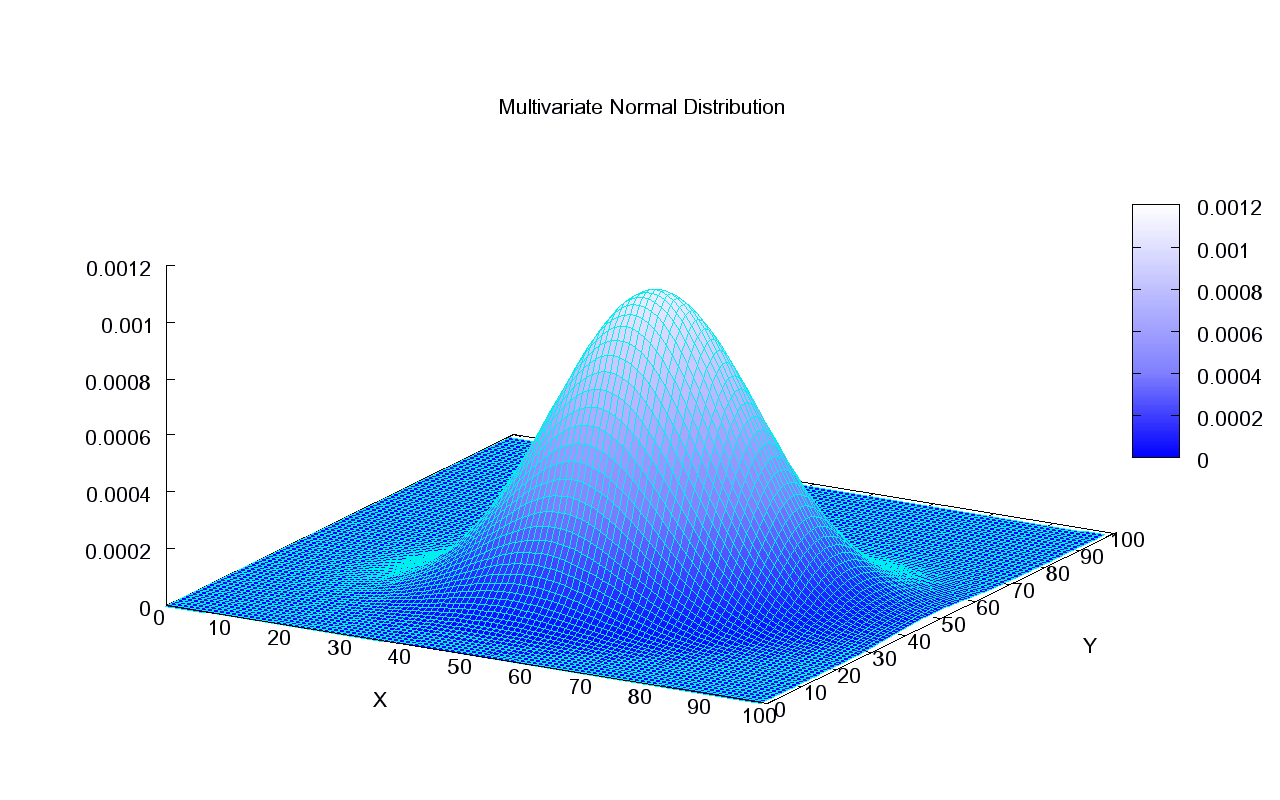
\includegraphics[width=\textwidth]{images/multi.png}
                \caption{$D = 2$}                
        \end{subfigure}    
        \begin{subfigure}[b]{0.23\textwidth}
                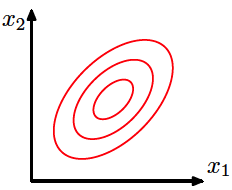
\includegraphics[width=\textwidth]{images/gnormal.png}
                \caption{}     
        \end{subfigure}
        \begin{subfigure}[b]{0.23\textwidth}
                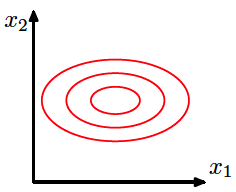
\includegraphics[width=\textwidth]{images/dnormal.png}
                \caption{$\mathbf{\Sigma} = \text{diag}(\sigma_i)$}
        \end{subfigure}
        \begin{subfigure}[b]{0.23\textwidth}
                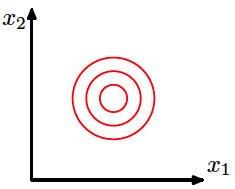
\includegraphics[width=\textwidth]{images/enormal.png}
                \caption{$\mathbf{\Sigma} = \sigma I$}
        \end{subfigure}
\end{figure}

\end{frame}

\begin{frame}{Old Faithful data set}

\begin{quote}
D = date of recordings in month (in August) \\
X = duration of the current eruption in minutes \\
Y = waiting time until the next eruption in minutes \\
\end{quote}

\begin{figure}
        \centering
        \begin{subfigure}[b]{0.33\textwidth}
                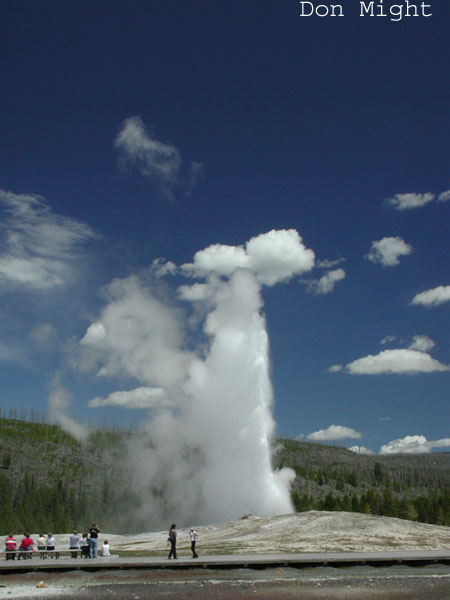
\includegraphics[width=\textwidth]{images/of1.jpg}
                \caption{Yellowstone Park}                
        \end{subfigure}    
        \begin{subfigure}[b]{0.6\textwidth}
                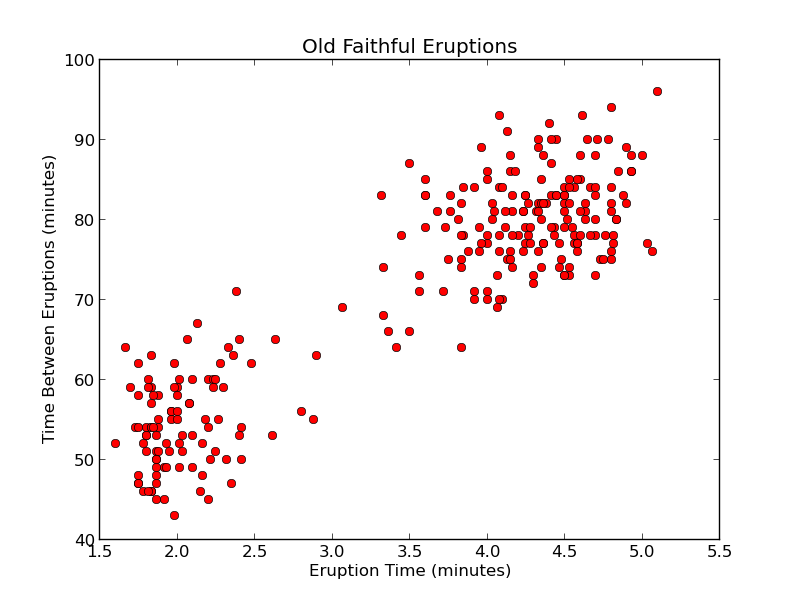
\includegraphics[width=\textwidth]{images/of2.png}
                \caption{}
        \end{subfigure}        
\end{figure}

\end{frame}

\begin{frame}{Смесь нормальных распределений}

``Скрытая'' $K$-мерная переменная $\mathbf{z}$ -- принадлежность объекта к одному из кластеров
\[
p(z_k = 1) = \pi_k, \quad z_k \in \{0, 1\}, \quad \sum_k z_k = 1 \quad\rightarrow\quad p(\mathbf{z}) = \prod_k \pi_k^{z_k}
\]

Распределение $\mathbf{x}$ для каждого из $K$ кластеров
\[
p(\mathbf{x} | \mathbf{z_k}) = \mathcal{N}(\mathbf{x} | \mathbf{\mu}_k, \mathbf{\Sigma}_k) \quad \rightarrow \quad p(\mathbf{x} | \mathbf{z}) = \prod_k \mathcal{N}(\mathbf{x} | \mathbf{\mu}_k, \mathbf{\Sigma}_k)^{z_k}
\]
Смесь нормальных распределений
\[
p(\mathbf{x}) = \sum_k \pi_k \mathcal{N}(\mathbf{x} | \mathbf{\mu}_k, \mathbf{\Sigma}_k)
\]

\end{frame}

\begin{frame}{}

Апостериорная вероятность принадлежности к $k$ кластеру (априорная равна $\pi_k$)
\[
\gamma(z_k) = p(z_k = 1 | \mathbf{x}) = \frac{p(z_k=1) p(\mathbf{x} | z_k = 1)}{\sum_{j=1}^K p(z_j=1) p(\mathbf{x} | z_j = 1)} =
\]
\[
= \frac{\pi_k \mathcal{N}(\mathbf{x} | \mathbf{\mu}_k, \mathbf{\Sigma}_k)}{\sum_{j=1}^K \pi_j \mathcal{N}(\mathbf{x} | \mathbf{\mu}_j, \mathbf{\Sigma}_j)}
\]

\end{frame}

\begin{frame}{Maximum Likelihood (!)}

\begin{block}{ML принцип}
Пусть дано семейство параметрических моделей $h(\mathbf{x}, \mathbf{\theta})$. Выбираем вектор параметров $\theta$, максимизирующий функцию правдоподобия (likelihood) $p(\mathcal{D} | \theta)$, соответствующую рассматриваемому семейству моделей.
\end{block}

\vspace{1em}
Функция правдоподобия
\[
\log(\mathbf{X} | \mathbf{\pi}, \mathbf{\mu}, \mathbf{\Sigma}) = \sum_{n=1}^N \log \sum_k \pi_k \mathcal{N}(\mathbf{x}_n | \mathbf{\mu}_k, \mathbf{\Sigma}_k) \rightarrow \max_{\mathbf{\pi}, \mathbf{\mu}, \mathbf{\Sigma}}
\]

Сложности
\begin{itemize}
\item схлопывание компонент
\item переименование кластеров
\item невозможно оптимизировать аналитически
\end{itemize}

\end{frame}

\begin{frame}{}

Дифференцируем функцию правдоподобия
\[
N_k = \sum_{n=1}^N \gamma(z_{nk}), \;\; \mu_k = \frac 1 {N_k} \sum_{n=1}^N \gamma(z_{nk}) \mathbf{x}_n
\]
\[
\Sigma_k = \frac 1 {N_k} \sum_{n=1}^N \gamma(z_{nk}) (\mathbf{x}_n - \mu_k)^T (\mathbf{x}_n - \mu_k)
\]
\[
\pi_k = \frac{N_k}{N}
\]

\end{frame}

\begin{frame}{Expectation Maximization (!)}

\begin{enumerate}
\item[E] Expectation: при фиксированных $\mu_k, \Sigma_k, \pi_k$
\[
\gamma(z_{nk}) = \frac{\pi_k \mathcal{N} (\mathbf{x}_n | \mu_k, \Sigma_k)}{\sum_{j=1}^K \pi_j \mathcal{N} (\mathbf{x}_n | \mu_j, \Sigma_j)}
\]
\item[M] Maximization: при фиксированных $\gamma(z_{nk})$
\[
N_k = \sum_{n=1}^N \gamma(z_{nk}), \;\; \mu_k = \frac 1 {N_k} \sum_{n=1}^N \gamma(z_{nk}) \mathbf{x}_n
\]
\[
\Sigma_k = \frac 1 {N_k} \sum_{n=1}^N \gamma(z_{nk}) (\mathbf{x}_n - \mu_k)(\mathbf{x}_n - \mu_k)^T
\]
\[
\pi_k = \frac{N_k}{N}
\]
\item[S] Остановиться при достижении сходимости
\end{enumerate}

\end{frame}

\begin{frame}{}

\begin{center}
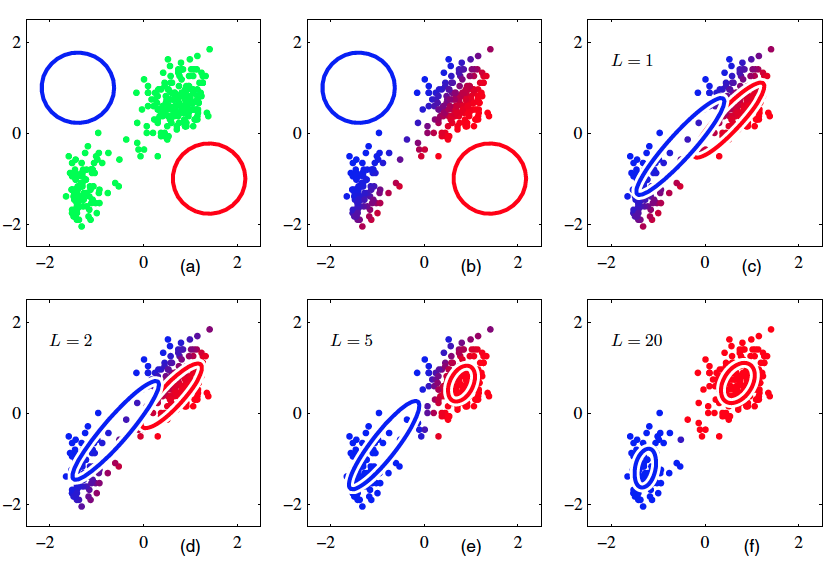
\includegraphics[scale=0.35]{images/gauss.png}
\end{center}

\end{frame}

\begin{frame}{EM-алгоритм}

{\bf Дано.} Известно распределение $P(\mathbf{X}, \mathbf{Z} | \theta)$, где $\mathbf{x}$ -- наблюдаемые переменные, а $\mathbf{z}$ -- скрытые. 

{\bf Найти.} $\theta$,  максимизирующее $P(\mathbf{X} | \theta)$.

\vspace{1em}
\begin{itemize}
\item[E] вычислить $P(\mathbf{Z} | \mathbf{X}, \theta^{old})$ при фиксированном $\theta^{old}$
\item[M] вычислить $\theta^{new} = \arg \max_{\theta} \mathcal{Q} (\theta, \theta^{old})$, где
\[
\mathcal{Q} (\theta, \theta^{old}) = E_\mathbf{Z}[\ln p(\mathbf{X}, \mathbf{Z} | \theta)] = \sum_{\mathbf{Z}} p(\mathbf{Z} | \mathbf{X}, \theta^{old}) \ln p(\mathbf{X}, \mathbf{Z} | \theta))
\]
\end{itemize}
{\it Улучшение:} ввести априорное распределение $p(\theta)$

\end{frame}

% =======================
\section{K-means и его модификации}
% =======================

\begin{frame}{K-means}

Пусть $\Sigma_k = \epsilon I$, тогда
\[
p(\mathbf{x} | \mu_k, \Sigma_k) = \frac{1}{\sqrt{2\pi\epsilon}}\exp(-\frac{1}{2\epsilon}\|\mathbf{x}-\mathbf{\mu_k}\|^2)
\]
Рассмотрим стремление $\epsilon \rightarrow 0$
\[
\gamma(z_{nk}) = \frac{\pi_k \exp(-\frac{1}{2\epsilon}\|\mathbf{x}_n-\mathbf{\mu_k}\|^2)}{\sum_j \pi_j \exp(-\frac{1}{2\epsilon}\|\mathbf{x}_n-\mathbf{\mu_j}\|^2)} \rightarrow r_{nk} = \begin{cases}
1, \; \text{для } k = \arg \min_j \|\mathbf{x}_n - \mathbf{\mu_j}\|^2 \\
0, \; \text{иначе}
\end{cases}
\]
Функция правдоподобия
\[
E_\mathbf{Z}[\ln p(\mathbf{X}, \mathbf{Z} | \mu, \Sigma, \pi)] \rightarrow -\sum_{n=1}^N \sum_{k=1}^K r_{nk} \| \mathbf{x}_n - \mu_k \|^2 + const
\]
Вектор средних
\[
\mathbf{\mu}_k = \frac{\sum_n r_{nk} \mathbf{x_n}}{\sum_n r_{nk}} 
\]

\end{frame}

\begin{frame}{K-means}

\kmeans
Сложность $O(NK)$ \\
Локальная оптимизация (!)

\end{frame}

\begin{frame}{}

\begin{center}
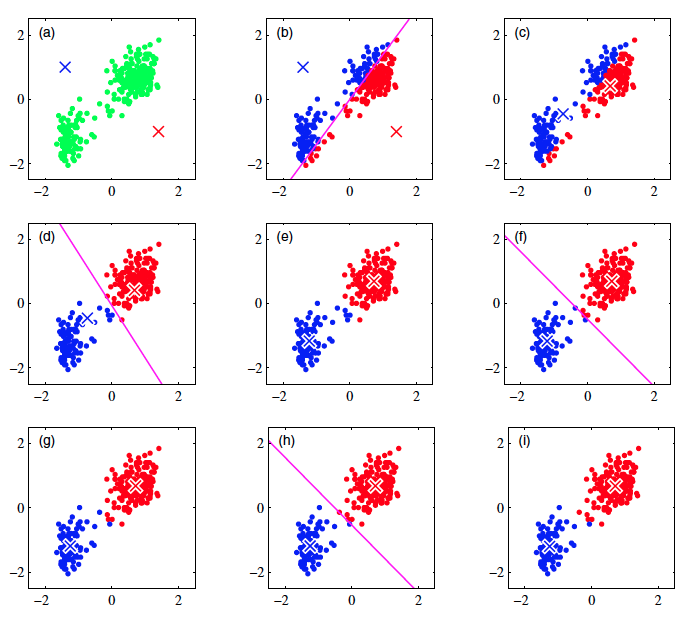
\includegraphics[scale=0.35]{images/kmeans.png}
\end{center}

\end{frame}

\begin{frame}{Задача}

\begin{center}
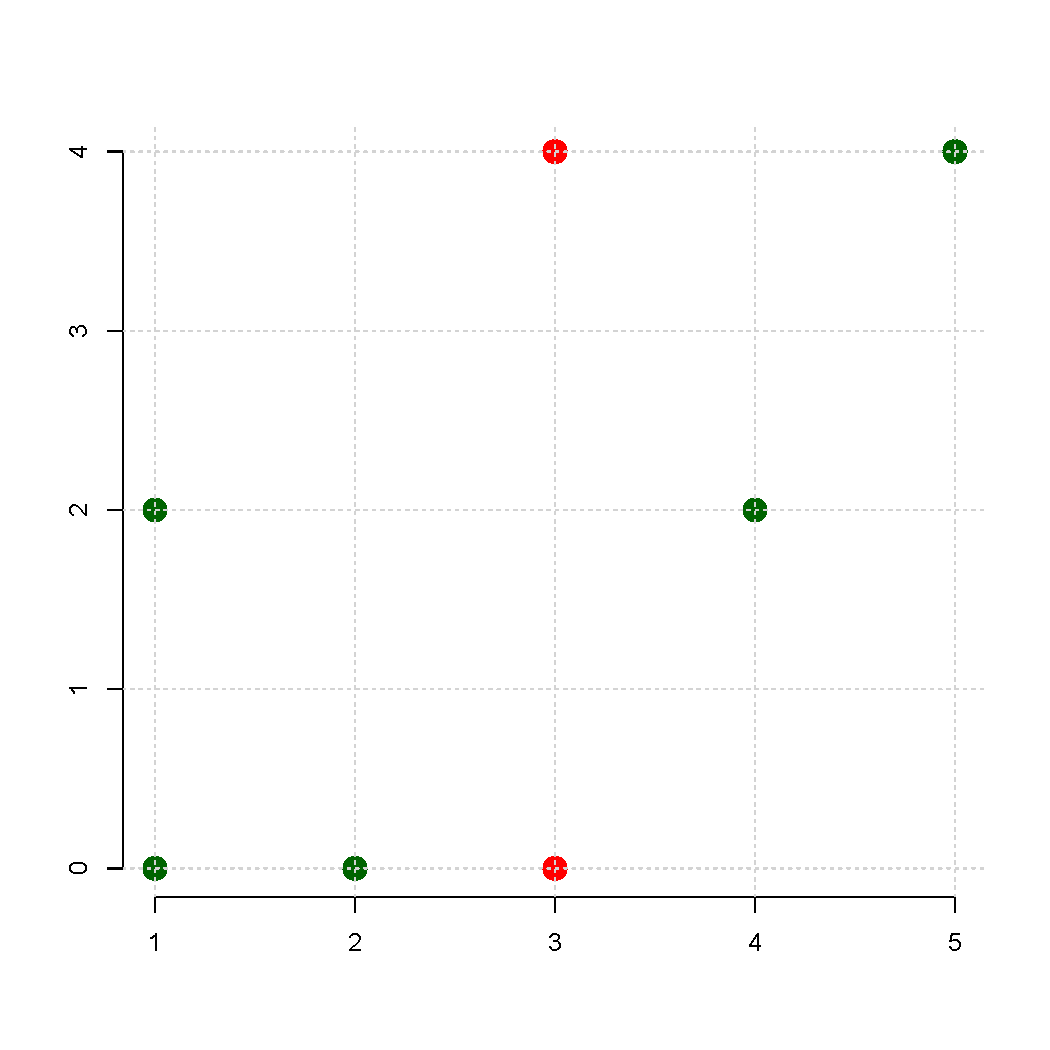
\includegraphics[height=0.9\textheight]{images/problem.pdf}
\end{center}

\end{frame}

\begin{frame}{Модификации k-means}

\begin{itemize}
\item На каждом шаге работаем с $b$ случайно выбранными объектами из каждого кластера (mini-batch k-means) \\
\begin{center}
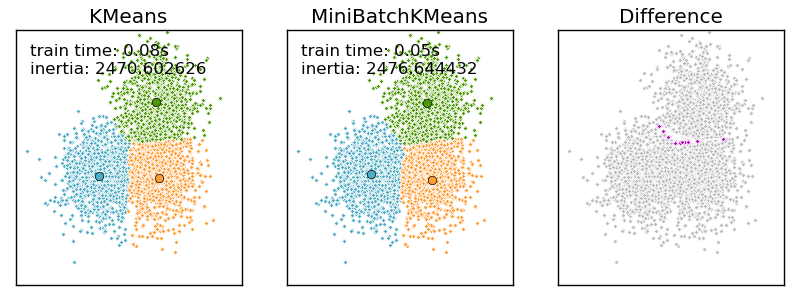
\includegraphics[scale=0.35]{images/mbatch.png}
\end{center}
\item Критерий качества (k-medoids)
\[
\tilde J = \sum_{n=1}^N \sum_{k=1}^K r_{nk} d(\mathbf{x}_n, \mu_k)
\]
$d$ -- функция расстояния, $\mu_k$ -- один из объектов в кластере
\end{itemize}

\end{frame}

\begin{frame}{Альтернативные функции расстояния}

\begin{exampleblock}{Def}
Функция $d(\mathbf{x}, \mathbf{y}): \mathbf{X} \times \mathbf{X} \rightarrow R$ является функцией расстояния, определенной на пространстве $\mathbf{X}$ тогда и только тогда, когда $\forall \mathbf{x} \in \mathbf{X}, \; \forall \mathbf{y} \in \mathbf{X}, \; \forall \mathbf{z} \in \mathbf{X}$ выполнено:
\begin{enumerate}
\item $d(\mathbf{x}, \mathbf{y}) \geq 0$
\item $d(\mathbf{x}, \mathbf{y}) = 0 \Leftrightarrow \mathbf{x} = \mathbf{y}$
\item $d(\mathbf{x}, \mathbf{y}) = d(\mathbf{y}, \mathbf{x})$
\item $d(\mathbf{x}, \mathbf{y}) \leq d(\mathbf{x}, \mathbf{z}) + d(\mathbf{y}, \mathbf{z})$
\end{enumerate}
\end{exampleblock}

\end{frame}

\begin{frame}{Расстояния 1}

\begin{columns}[T]
    \begin{column}{.5\textwidth}
    \begin{itemize}
		\item Минковского
		\[
		d_r(\mathbf{x}, \mathbf{y}) = \left[ \sum_{j=1}^N |x_j - y_j|^r \right]^{\frac{1}{r}}
		\]
		\item Евклидово $r = 2$
		\[
		d_E(\mathbf{x}, \mathbf{y}) = d_2(\mathbf{x}, \mathbf{y})
		\]
		\item Манхэттэн $r = 1$
		\[
		d_M(\mathbf{x}, \mathbf{y}) = d_1(\mathbf{x}, \mathbf{y})
		\]
		\item $r=\infty$
		\[
		d_\infty(\mathbf{x}, \mathbf{y}) = \max_j |x_j - y_j|
		\]
	\end{itemize}
    \end{column}
       
    \begin{column}{.5\textwidth}
    \vspace{2em}
	\begin{center}
   		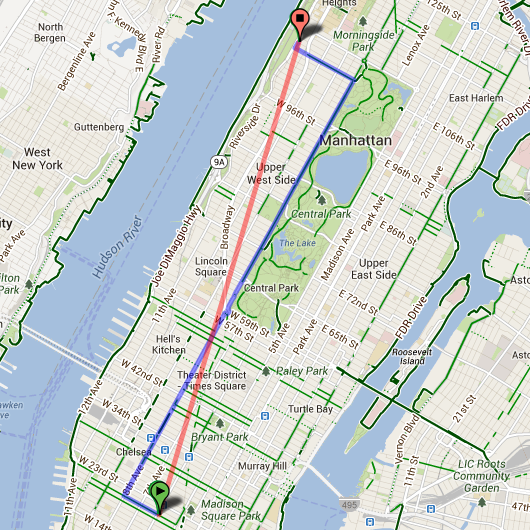
\includegraphics[scale=0.25]{images/manhattan.png}
    \end{center}
    \end{column}
  \end{columns}

\end{frame}

\begin{frame}{Проблема}

Функции расстояния чувствительны к преобразоаниям данных

\vspace{1em}
Решение
\begin{itemize}
\item Преобразовать обучающую выборку так, чтобы  признаки имели нулевое среднее и единичную дисперсию -- инвариантность к растяжению и сдвигу (standartize)
\item Преобразовать обучающую выборку так, чтобы оси совпадали с главными компонентами матрицы ковариации -- инвариантность относительно поворотов (PCA)
\end{itemize}


\end{frame}

\begin{frame}{Расстояния 2}

\begin{columns}[T]

    \begin{column}{.4\textwidth}
    \vspace{5em}
	\begin{center}
   		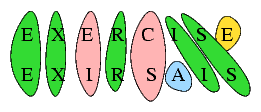
\includegraphics[scale=0.5]{images/edit.png}
    \end{center}
    \end{column}
       
    \begin{column}{.6\textwidth}
    \begin{itemize}
		\item Жаккар
		\[
		d_J(\mathbf{x}, \mathbf{y}) = 1 - \frac{|\mathbf{x} \cap \mathbf{y}|}{|\mathbf{x} \cup \mathbf{y}|}
		\]
		\item Косинус
		\[
		d_c(\mathbf{x}, \mathbf{y}) = \arccos \frac{\mathbf{x} \mathbf{y}}{\|\mathbf{x}\| \|\mathbf{y}\|}
		\]
		\item Правки \\
		{\it $d_e$ -- наименьшее количество удалений и вставок, приводящее $\mathbf{x}$ к $\mathbf{y}$.}
		\item Хэмминг \\
		{\it $d_H$ -- количество различных компонент в $\mathbf{x}$ и $\mathbf{y}$.}
	\end{itemize}
    
    \end{column}
  \end{columns}

\end{frame}

\begin{frame}{Проклятие размерности}

\begin{block}{Задача}
Даны два случайных вектора $\mathbf{x}$ и $\mathbf{y}$ в пространстве размерности $D$. Как зависит математическое ожидание косинус-расстояния между $\mathbf{x}$ и $\mathbf{y}$ от размерности $D$?
\end{block}

\[
d_c(\mathbf{x}, \mathbf{y}) = \arccos \frac{\sum_{j=1}^D x_j y_j}{\sum_{j=1}^D x_j^2 \sum_{j=1}^D y_j^2}
\]
Наблюдения:
\begin{itemize}
\item числитель стремится к нулю
\item знаменатель положительный
\end{itemize}
Вывод: $d_c(\mathbf{x}, \mathbf{y}) \rightarrow \frac \pi 2$.

\end{frame}

\begin{frame}{Альтернативные критерии качества}

Критерий
\begin{eqnarray*}
J &=& \sum_{k=1}^K \sum_{\mathbf{x}_i \in C_k} \| \mathbf{x}_i - \mathbf{m}_k \|^2 = \\
&=& \frac 1 2 \sum_{k=1}^K n_k \left[ \frac{1}{n_k^2} \sum_{\mathbf{x}_i \in C_k} \sum_{\mathbf{x}_j \in C_k} \| \mathbf{x}_i - \mathbf{x}_j \|^2 \right] = \\
&=& \frac 1 2 \sum_{k=1}^K n_k \left[ \frac{1}{n_k^2} \sum_{\mathbf{x}_i \in C_k} \sum_{\mathbf{x}_j \in C_k} s(\mathbf{x}_i, \mathbf{x}_j) \right] = \frac 1 2 \sum_{k=1}^K n_k \bar s_k
\end{eqnarray*}
Примеры $\bar s_i$
\[
\underline{s}_k = \min_{\mathbf{x}_i, \mathbf{x}_j} s(\mathbf{x}_i, \mathbf{x}_j); \quad \bar s_k = \max_{\mathbf{x}_i, \mathbf{x}_j} s(\mathbf{x}_i, \mathbf{x}_j)\]

\end{frame}

\begin{frame}{Кластеризация}

\begin{block}{Идея}
Выбрать критерий качества кластеризации $J$ и расстояние между объектами $d(\mathbf{x}_i, \mathbf{x}_j)$ и вычислить разбиение выборки на кластеры, которое которое соответствует оптимальному значению выбранного критерия.
\end{block}

\end{frame}

\begin{frame}{Качество кластеризации}

Пусть дана обучающая выборка, для которой правильная кластеризация $C$ известна. С помощью выбранного алгоритма получена кластеризация $K$. Проверить, насколько $K$ совпадает с $C$.

\vspace{1em}
\begin{itemize}
\item Rand Index \\
{\it \small
$a$ -- кол-во пар объектов, попавших в один кластер и в $C$, и в $K$ \\
$b$ -- кол-во пар объектов, попавших в разные кластеры и в $C$, и в $K$
\[
RI = \frac{a+b}{C^N_2}
\]
}
\item Mutual Information \\
{\it \small
\[
MI = \sum_{c \in C} \sum_{k \in K} p(c, k) \log \frac{p(c, k)}{p(k)p(c)}
\]
}
\end{itemize}

\end{frame}

\begin{frame}[fragile]{Задача}

{\bf Дано:} Сгенерированная смесь из гауссовских распределений \\
{\bf Требуется:} Исследовать стабильность и чувствительность к линейным преобразованиям алгоритма k-means

\vspace{1em}
Пошаговая инструкция
\begin{enumerate}
\item Скачать и запустить шаблон кода на python \url{http://bit.ly/1yyVTyw}
\begin{shaded}
{\color{green} \begin{verbatim}
$ python kmeans.py -h
$ python kmeans.py
\end{verbatim}}
\end{shaded}
\item Заполнить функцию \textsf{rand\_index} \\ Меняется ли rand от запуска к запуску?
\item Дописать функцию \textsf{cluster\_data} \\ Реализовать N-times random restart
\item Как меняется результат кластеризации, если применить к данным различные линейные преобразования?
\end{enumerate}

\end{frame}

\begin{frame}[plain]
\begin{center}
{\Large Вопросы}
\end{center}
\end{frame}

\end{document}